% no answer key
% \documentclass[letterpaper]{exam}

% answer key
\documentclass[letterpaper, landscape]{exam}
\usepackage{2in1, lscape} 
\printanswers

\usepackage{units} 
\usepackage{xfrac} 
\usepackage[fleqn]{amsmath}
\usepackage{float}
\usepackage{mdwlist}
\usepackage{booktabs}
\usepackage{cancel}
\usepackage{polynom}
\usepackage{caption}
\usepackage{fullpage}
\usepackage{comment}
\usepackage{enumerate}
\usepackage{graphicx}

\usepackage{mathtools} 

\newcommand{\dg}{\ensuremath{^\circ}} 
\newcommand{\sgn}{\operatorname{sgn}}

\everymath{\displaystyle}
\title{Calculus I \\ Homework Seven \\ Section 2.7}
\author{}
\date{\today}

\begin{document}

  \maketitle

  \section{Homework}
    \begin{itemize*}
      \item read Section 2.7
      \item exercises: 1, 5-8, 13-15, 18-19, 21-22, 25-32, 37-38, 40, 43, 46
    \end{itemize*}

  \ifprintanswers

  \section{Solutions}

    \begin{description}

      \item[1] 
        \begin{enumerate}[(a)]

          \item $m_{secant} = \frac{f(x) - f(3)}{x - 3}$ 

          \item $m_{tangent} = \lim_{x \to 3} \frac{f(x) - f(3)}{x - 3}$ 

        \end{enumerate}

      % \item[3]
      %   \begin{enumerate}[(a)]

      %     \item 
      %       \[
      %         m = \lim_{x \to 1} \frac{ 4x - x^2 - 3}{x - 1} = \boxed{ 2 }
      %       \]

      %     \item 
      %       \[
      %         m = \lim_{h \to 0} \frac{ 4 (1 + h) - (1 + h) ^2 - 3}{h} = \boxed{ 2 }
      %       \]
      %   \end{enumerate}

      \item[5]

        \begin{align*}
          f'(3) & = \lim_{x \to 3} \frac{ \left( \cfrac{x - 1}{x - 2} - 2 \right) }{x - 3}
          \\    & = -1 \\
          \\
          -1    & = \frac{y - 2}{x - 3} \\
          y     & = -x + 5 \\
        \end{align*}
          

      \item[6]
        \begin{align*}
          f'(-1) & = \lim_{x \to -1} \frac{ \left(  2x^3 - 5x \right) - 3 }{x - (-1)} \\
                 & = 1 \\
          \\
          1      & = \frac{y - 3}{x - (-1)} \\
          y      & = x + 4 \\
        \end{align*}

      \item[7]
        \begin{align*}
          f'(1)       & = \lim_{x \to 1} \frac{\sqrt{x} - 1 }{x - 1} \\
                      & = \frac{1}{2} \\
          \\
          \frac{1}{2} & = \frac{y - 1}{x - 1} \\
          y           & = \frac{x}{2} + \frac{1}{2} \\
        \end{align*}

      \item[8]
        \begin{align*}
          f'(0) & = \lim_{x \to 0} \frac{ \left( \cfrac{2x}{(x + 1)^2} - 0 \right) }{x - 0} \\
                & = 2 \\
          \\
          2     & = \frac{y - 0}{x - 0} \\
          y     & = 2x \\
        \end{align*}
      
      \item[13]
        \begin{align*}
          v & = \lim_{h \to 0} \frac{ 40(2 + h) - 16 (2 + h)^2 - \left( 40 \cdot 2 - 16 \cdot 2^2 \right)}{h} \\
            & = \boxed{ \unit[-24]{ft/s} }
        \end{align*}

      \item[14]
        \begin{enumerate}[(a)]
          \item 
            \begin{align*}
              v & = \lim_{h \to 0} \frac{ 10(1 + h) - 1.86 (1 + h)^2 - \left( 10 \cdot 1 - 1.86 \cdot 1^2 \right) }{h} \\
                & = \boxed{ \unit[6.28]{m/s} }
            \end{align*}

          \item
            \begin{align*}
              v & = \lim_{h \to 0} \frac{ 10(a + h) - 1.86 (a + h)^2 - \left( 10 a - 1.86 a^2 \right) }{h} \\
                & = \boxed{ 10 - 3.72a }
            \end{align*}

          \item
            \begin{align*}
              10t - 1.86t^2 & = 0 \\
              t             & \approx \boxed{ \unit[5.38]{s} } \\
            \end{align*}

          \item
            \[
              10 - 3.72 \cdot 5.38 \approx \boxed{ \unit[-10]{m/s} }
            \]

        \end{enumerate}

      \item[15]
        \begin{align*}
          f'(a) & = \lim_{x \to a} \frac{ 1/x^2 - 1/a^2}{x - a} \\
                & = \lim_{x \to a} \frac{ a^2 - x^2}{x^2a^2 (x - a)} \\
                & = - \lim_{x \to a} \frac{ x + a}{x^2a^2} \\
                & = \boxed{ \unit[- \frac{2}{a^3}]{m/s} } \\
          \\
          f'(1) & = -2 \\
          f'(2) & = - \frac{1}{4} \\
          f'(3) & = - \frac{2}{27} \\
        \end{align*}

      \newpage

      \item[18]
        \begin{enumerate}[(a)]

          \item 
            \begin{align*}
              4 & = \frac{y - (-3)}{x - 5} \\
              y & = 4x - 23 \\
            \end{align*}

          \item Since the point is $(4, 3)$, $f(4) = 3$

            The derivative is the same as the slope of the tangent line:
            \begin{align*}
              f'(4) & = \frac{3 - 2}{4 - 0} \\
                    & = \boxed{ \frac{1}{4} } \\
            \end{align*}

        \end{enumerate}

      \item[19] $f(0) = 0$, $f'(0) = 3$, $f'(1) = 0$ and $f'(2) = -1$
        
        \begin{figure}[H]
          \centering
          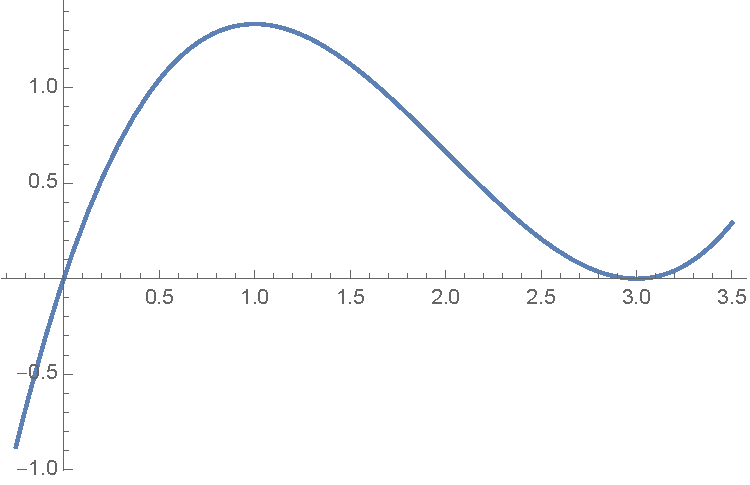
\includegraphics[scale = 0.5]{ex19.pdf}
          \caption{Exercise 19}
          \label{fig:ex19}
        \end{figure}

      \item[21] 
        \begin{align*}
          f'(2) & = \lim_{h \to 0} \frac{3 (2 + h)^2 - 5(2 + h) - \left( 2^2 - 5 \cdot 2 \right)}{h} \\
                & = 7 \\
          \\
          7     & = \frac{y - 2}{x - 2} \\
          y     & = 7x - 12 \\
        \end{align*}
 
      \item[22] 
        \begin{align*}
          f'(0) & = \lim_{h \to 0} \frac{1 - (0 + h)^3 - \left( 1 - 0^3 \right)}{h} \\
                & = 0 \\
          \\
          0     & = \frac{y - 1}{x - 0} \\
          y     & = 1 \\
        \end{align*}
 
      \item[25]
        \begin{align*}
          f'(a) & =\lim_{h \to 0} \frac{3 - 2(a + h) + 4 \left( a + h \right)^2 - \left( 3 - 2a - 4a^2 \right)}{h} \\
                & = \boxed{ 8a - 2 } \\
        \end{align*}

      \item[26]
        \begin{align*}
          f'(a) & = \lim_{h \to 0} \frac{ (a + h)^4 - 5(a + h) - \left( a^4 - 5a \right)}{h} \\
                & = \boxed{ 4a^3 - 5 } \\
        \end{align*}
 
      \item[27]
        \begin{align*}
          f'(a) & = \lim_{h \to 0} \frac{ \cfrac{2(a + h) + 1}{a + h + 3} - \cfrac{2a + 1}{a + 3}}{h} \\
                & = \boxed{ \frac{5}{(a + 3)^2} } \\
        \end{align*}
 
      \item[28]
        \begin{align*}
          f'(a) & = \lim_{h \to 0} \frac{ \cfrac{(a + h)^2 + 1}{a + h - 2} - \cfrac{a^2 + 1}{a - 2}}{h} \\
                & = \boxed{ \frac{a^2 - 4a - 1}{(a - 2)^2} } \\
        \end{align*}

      \item[29]
        \begin{align*}
          f'(a) & = \lim_{h \to 0} \frac{ \cfrac{1}{\sqrt{a + h + 2}} - \cfrac{1}{\sqrt{a + 2}}}{h} \\
                & = \boxed{ \frac{-1}{2(a + 2)^{3/2}} } \\
        \end{align*}

      \item[30]
        \begin{align*}
          f'(a) & = \lim_{h \to 0} \frac{ \sqrt{3(a + h) + 1} - \sqrt{3a + 1} }{h} \\
                & = \boxed{ \frac{3}{2 \sqrt{3a + 1}} } \\
        \end{align*}

      \item[31]
        \begin{align*}
          f(x) & = x^{10} \\
          a    & = 1 \\
        \end{align*}

      \item[32]
        \begin{align*}
          f(x) & = \sqrt[4]{x} \\
          a    & = 16 \\
        \end{align*}

      \item[37]
        \[
          v(5) = f'(5) = \boxed{\unit[1]{m/s}} 
        \]

        The speed is the absolute value of the velocity so it is also $\unit[1]{m/s}$ in this case.

      \item[38]
        \begin{align*}
          f'(t) & = - \frac{1}{t^2} - 1 \\
          f'(5) & = \boxed{ \unit[ - \frac{26}{25} ]{m/s} }
        \end{align*}

        The speed is the absolute value of the velocity so it is $\unit[\frac{26}{25} ]{m/s}$ in this case.
 
      \item[40]
        After an hour, the rate looks like about $\boxed{ - \unit[50]{degrees/hour} }$

      \newpage

      \item[43]
        \begin{enumerate}[(a)]
          \item 
            \begin{align*}
              r(100, 105) &= \frac{ C(105) - C(100) }{ 105 - 100 } = \unit[20.25]{\$/unit} \\
              r(100, 101) &= \frac{ C(101) - C(100) }{ 101 - 100 } = \unit[20.05]{\$/unit} \\
            \end{align*}

          \item
            \[
              C'(100) = \boxed{ \unit[20]{\$/unit} }
            \]
        \end{enumerate}

      \item[46]
        \begin{enumerate}[(a)]
          \item $f'(5)$ is the rate of change of bacteria after 5 hours in bacteria per hour.

          \item Since bacteria reproduce by splitting into two bacteria, the more of them
            there are, the higher the rate of change of bacteria, as long as there is
            unlimited space and food. $f'(10)$ will be larger than $f'(5)$ in these
            conditions.

            If the resources are limited, then at some point the bacteria will eat all the
            food, stop reproducing, and die out. The rate of change will eventually be
            negative, and then it will go to zero after all the bacteria are gone. 

        \end{enumerate}
     \end{description}
 
 
  \else
    \vspace{10 cm}
    \begin{quote}
      \begin{em}
        Your vision will become clear only when you look into your heart \dots Who looks
        outside, dreams. Who looks inside, awakens.
      \end{em}
    \end{quote}
    \hspace{2 cm} --Carl Jung
  \fi

\end{document}

